\documentclass[twoside]{book}

% Packages required by doxygen
\usepackage{fixltx2e}
\usepackage{calc}
\usepackage{doxygen}
\usepackage[export]{adjustbox} % also loads graphicx
\usepackage{graphicx}
\usepackage[utf8]{inputenc}
\usepackage{makeidx}
\usepackage{multicol}
\usepackage{multirow}
\PassOptionsToPackage{warn}{textcomp}
\usepackage{textcomp}
\usepackage[nointegrals]{wasysym}
\usepackage[table]{xcolor}

% Font selection
\usepackage[T1]{fontenc}
\usepackage[scaled=.90]{helvet}
\usepackage{courier}
\usepackage{amssymb}
\usepackage{sectsty}
\renewcommand{\familydefault}{\sfdefault}
\allsectionsfont{%
  \fontseries{bc}\selectfont%
  \color{darkgray}%
}
\renewcommand{\DoxyLabelFont}{%
  \fontseries{bc}\selectfont%
  \color{darkgray}%
}
\newcommand{\+}{\discretionary{\mbox{\scriptsize$\hookleftarrow$}}{}{}}

% Page & text layout
\usepackage{geometry}
\geometry{%
  a4paper,%
  top=2.5cm,%
  bottom=2.5cm,%
  left=2.5cm,%
  right=2.5cm%
}
\tolerance=750
\hfuzz=15pt
\hbadness=750
\setlength{\emergencystretch}{15pt}
\setlength{\parindent}{0cm}
\setlength{\parskip}{3ex plus 2ex minus 2ex}
\makeatletter
\renewcommand{\paragraph}{%
  \@startsection{paragraph}{4}{0ex}{-1.0ex}{1.0ex}{%
    \normalfont\normalsize\bfseries\SS@parafont%
  }%
}
\renewcommand{\subparagraph}{%
  \@startsection{subparagraph}{5}{0ex}{-1.0ex}{1.0ex}{%
    \normalfont\normalsize\bfseries\SS@subparafont%
  }%
}
\makeatother

% Headers & footers
\usepackage{fancyhdr}
\pagestyle{fancyplain}
\fancyhead[LE]{\fancyplain{}{\bfseries\thepage}}
\fancyhead[CE]{\fancyplain{}{}}
\fancyhead[RE]{\fancyplain{}{\bfseries\leftmark}}
\fancyhead[LO]{\fancyplain{}{\bfseries\rightmark}}
\fancyhead[CO]{\fancyplain{}{}}
\fancyhead[RO]{\fancyplain{}{\bfseries\thepage}}
\fancyfoot[LE]{\fancyplain{}{}}
\fancyfoot[CE]{\fancyplain{}{}}
\fancyfoot[RE]{\fancyplain{}{\bfseries\scriptsize Generated by Doxygen }}
\fancyfoot[LO]{\fancyplain{}{\bfseries\scriptsize Generated by Doxygen }}
\fancyfoot[CO]{\fancyplain{}{}}
\fancyfoot[RO]{\fancyplain{}{}}
\renewcommand{\footrulewidth}{0.4pt}
\renewcommand{\chaptermark}[1]{%
  \markboth{#1}{}%
}
\renewcommand{\sectionmark}[1]{%
  \markright{\thesection\ #1}%
}

% Indices & bibliography
\usepackage{natbib}
\usepackage[titles]{tocloft}
\setcounter{tocdepth}{3}
\setcounter{secnumdepth}{5}
\makeindex

% Hyperlinks (required, but should be loaded last)
\usepackage{ifpdf}
\ifpdf
  \usepackage[pdftex,pagebackref=true]{hyperref}
\else
  \usepackage[ps2pdf,pagebackref=true]{hyperref}
\fi
\hypersetup{%
  colorlinks=true,%
  linkcolor=blue,%
  citecolor=blue,%
  unicode%
}

% Custom commands
\newcommand{\clearemptydoublepage}{%
  \newpage{\pagestyle{empty}\cleardoublepage}%
}

\usepackage{caption}
\captionsetup{labelsep=space,justification=centering,font={bf},singlelinecheck=off,skip=4pt,position=top}

%===== C O N T E N T S =====

\begin{document}

% Titlepage & ToC
\hypersetup{pageanchor=false,
             bookmarksnumbered=true,
             pdfencoding=unicode
            }
\pagenumbering{alph}
\begin{titlepage}
\vspace*{7cm}
\begin{center}%
{\Large R\+Sym\+S\+Q\+CD }\\
\vspace*{1cm}
{\large Generated by Doxygen 1.8.13}\\
\end{center}
\end{titlepage}
\clearemptydoublepage
\pagenumbering{roman}
\tableofcontents
\clearemptydoublepage
\pagenumbering{arabic}
\hypersetup{pageanchor=true}

%--- Begin generated contents ---
\chapter{Hierarchical Index}
\section{Class Hierarchy}
This inheritance list is sorted roughly, but not completely, alphabetically\+:\begin{DoxyCompactList}
\item \contentsline{section}{C\+S\+Dipole}{\pageref{classCSDipole}}{}
\item \contentsline{section}{I\+Matrix\+Elements}{\pageref{classIMatrixElements}}{}
\begin{DoxyCompactList}
\item \contentsline{section}{M\+R\+S\+SM}{\pageref{classMRSSM}}{}
\item \contentsline{section}{M\+S\+SM}{\pageref{classMSSM}}{}
\item \contentsline{section}{SM}{\pageref{classSM}}{}
\end{DoxyCompactList}
\item \contentsline{section}{Process}{\pageref{classProcess}}{}
\item \contentsline{section}{Vec4D$<$ T $>$}{\pageref{classVec4D}}{}
\item \contentsline{section}{X\+Section}{\pageref{classXSection}}{}
\begin{DoxyCompactList}
\item \contentsline{section}{X\+Section\+\_\+\+HnonC}{\pageref{classXSection__HnonC}}{}
\item \contentsline{section}{X\+Section\+\_\+\+SC}{\pageref{classXSection__SC}}{}
\item \contentsline{section}{X\+Section\+\_\+\+Tree}{\pageref{classXSection__Tree}}{}
\item \contentsline{section}{X\+Section\+\_\+\+Virt}{\pageref{classXSection__Virt}}{}
\end{DoxyCompactList}
\end{DoxyCompactList}

\chapter{Class Index}
\section{Class List}
Here are the classes, structs, unions and interfaces with brief descriptions\+:\begin{DoxyCompactList}
\item\contentsline{section}{\hyperlink{classCSDipole}{C\+S\+Dipole} }{\pageref{classCSDipole}}{}
\item\contentsline{section}{\hyperlink{classIMatrixElements}{I\+Matrix\+Elements} }{\pageref{classIMatrixElements}}{}
\item\contentsline{section}{\hyperlink{classMRSSM}{M\+R\+S\+SM} }{\pageref{classMRSSM}}{}
\item\contentsline{section}{\hyperlink{classMSSM}{M\+S\+SM} }{\pageref{classMSSM}}{}
\item\contentsline{section}{\hyperlink{classProcess}{Process} }{\pageref{classProcess}}{}
\item\contentsline{section}{\hyperlink{classSM}{SM} }{\pageref{classSM}}{}
\item\contentsline{section}{\hyperlink{classVec4D}{Vec4\+D$<$ T $>$} }{\pageref{classVec4D}}{}
\item\contentsline{section}{\hyperlink{classXSection}{X\+Section} }{\pageref{classXSection}}{}
\item\contentsline{section}{\hyperlink{classXSection__HnonC}{X\+Section\+\_\+\+HnonC} }{\pageref{classXSection__HnonC}}{}
\item\contentsline{section}{\hyperlink{classXSection__SC}{X\+Section\+\_\+\+SC} }{\pageref{classXSection__SC}}{}
\item\contentsline{section}{\hyperlink{classXSection__Tree}{X\+Section\+\_\+\+Tree} }{\pageref{classXSection__Tree}}{}
\item\contentsline{section}{\hyperlink{classXSection__Virt}{X\+Section\+\_\+\+Virt} }{\pageref{classXSection__Virt}}{}
\end{DoxyCompactList}

\chapter{Class Documentation}
\hypertarget{classCSDipole}{}\section{C\+S\+Dipole Class Reference}
\label{classCSDipole}\index{C\+S\+Dipole@{C\+S\+Dipole}}
\subsection*{Public Member Functions}
\begin{DoxyCompactItemize}
\item 
\mbox{\Hypertarget{classCSDipole_ae83f860e66196eead00bf2f8e82a0c49}\label{classCSDipole_ae83f860e66196eead00bf2f8e82a0c49}} 
{\bfseries C\+S\+Dipole} (boost\+::property\+\_\+tree\+::ptree pt, Dipole\+Type type, unsigned int i, unsigned int j)
\item 
\mbox{\Hypertarget{classCSDipole_adfd7fba72b9914ce8af7f9b7fd2adc28}\label{classCSDipole_adfd7fba72b9914ce8af7f9b7fd2adc28}} 
double {\bfseries eval\+\_\+unintegrated\+\_\+dipole} (std\+::vector$<$ \hyperlink{classVec4D}{Vec4D}$<$ double $>$$>$ const \&) const
\item 
\mbox{\Hypertarget{classCSDipole_a1505e9e1e6340264127bf773b911a0c9}\label{classCSDipole_a1505e9e1e6340264127bf773b911a0c9}} 
double {\bfseries eval\+\_\+integrated\+\_\+dipole} (int, std\+::vector$<$ \hyperlink{classVec4D}{Vec4D}$<$ double $>$$>$ const \&) const
\item 
\mbox{\Hypertarget{classCSDipole_ac24dc706498541f9c824b90c96780252}\label{classCSDipole_ac24dc706498541f9c824b90c96780252}} 
double {\bfseries eval\+\_\+P} (std\+::vector$<$ \hyperlink{classVec4D}{Vec4D}$<$ double $>$$>$ const \&, double) const
\item 
\mbox{\Hypertarget{classCSDipole_a4d81b94ed59dd5716e7966daf5b2516c}\label{classCSDipole_a4d81b94ed59dd5716e7966daf5b2516c}} 
double {\bfseries eval\+\_\+K} (std\+::vector$<$ \hyperlink{classVec4D}{Vec4D}$<$ double $>$$>$ const \&, double) const
\item 
\mbox{\Hypertarget{classCSDipole_a1eaaba4413e967b6e93a4b6bf24d3051}\label{classCSDipole_a1eaaba4413e967b6e93a4b6bf24d3051}} 
unsigned int {\bfseries get\+\_\+emitter} () const
\item 
\mbox{\Hypertarget{classCSDipole_a9dc70c81039b4b9b45c32462ec7dff7e}\label{classCSDipole_a9dc70c81039b4b9b45c32462ec7dff7e}} 
unsigned int {\bfseries get\+\_\+spectator} () const
\end{DoxyCompactItemize}
\subsection*{Public Attributes}
\begin{DoxyCompactItemize}
\item 
\mbox{\Hypertarget{classCSDipole_a0f5d6f5387740845f43b50d0faa9c61d}\label{classCSDipole_a0f5d6f5387740845f43b50d0faa9c61d}} 
\hyperlink{classIMatrixElements}{I\+Matrix\+Elements} const  $\ast$const {\bfseries model\+\_\+}
\end{DoxyCompactItemize}


The documentation for this class was generated from the following files\+:\begin{DoxyCompactItemize}
\item 
/home/wojciechk1/\+Programowanie/c++/rsymsqcd/include/C\+S\+Dipole.\+hpp\item 
/home/wojciechk1/\+Programowanie/c++/rsymsqcd/src/C\+S\+Dipole.\+cpp\end{DoxyCompactItemize}

\hypertarget{classIMatrixElements}{}\section{I\+Matrix\+Elements Class Reference}
\label{classIMatrixElements}\index{I\+Matrix\+Elements@{I\+Matrix\+Elements}}
Inheritance diagram for I\+Matrix\+Elements\+:\begin{figure}[H]
\begin{center}
\leavevmode
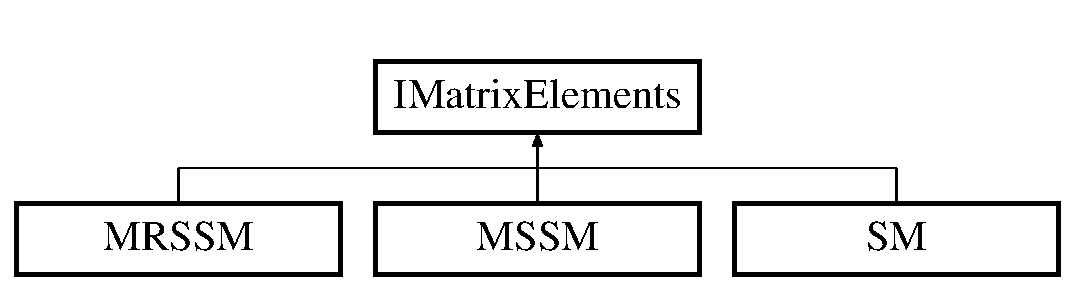
\includegraphics[height=2.000000cm]{classIMatrixElements}
\end{center}
\end{figure}
\subsection*{Public Member Functions}
\begin{DoxyCompactItemize}
\item 
\mbox{\Hypertarget{classIMatrixElements_a458dffa42a09708a69ba0aa7c6cb3476}\label{classIMatrixElements_a458dffa42a09708a69ba0aa7c6cb3476}} 
virtual double {\bfseries Born\+ME} (std\+::vector$<$ Particle $>$, double, double) const noexcept=0
\item 
\mbox{\Hypertarget{classIMatrixElements_a8db0be3169c7a298a3a839f705bd078a}\label{classIMatrixElements_a8db0be3169c7a298a3a839f705bd078a}} 
virtual double {\bfseries Born\+C\+C\+ME} (std\+::vector$<$ Particle $>$, int, int, Eps\+Ord, std\+::vector$<$ \hyperlink{classVec4D}{Vec4D}$<$ double $>$$>$ const \&) const noexcept=0
\item 
\mbox{\Hypertarget{classIMatrixElements_aec3e7e3b834a85e1db346fd5aaa53dae}\label{classIMatrixElements_aec3e7e3b834a85e1db346fd5aaa53dae}} 
virtual double {\bfseries Virtual\+ME} (std\+::vector$<$ Particle $>$, Eps\+Ord, double, double) const noexcept=0
\item 
\mbox{\Hypertarget{classIMatrixElements_a06fe3f65de1611596cb6e43c8168aa52}\label{classIMatrixElements_a06fe3f65de1611596cb6e43c8168aa52}} 
virtual double {\bfseries Real\+ME} (std\+::vector$<$ Particle $>$, std\+::vector$<$ \hyperlink{classVec4D}{Vec4D}$<$ double $>$$>$ const \&) const noexcept=0
\end{DoxyCompactItemize}
\subsection*{Static Public Member Functions}
\begin{DoxyCompactItemize}
\item 
\mbox{\Hypertarget{classIMatrixElements_af0cddd29f2a2d301f182509141a889ad}\label{classIMatrixElements_af0cddd29f2a2d301f182509141a889ad}} 
static \hyperlink{classIMatrixElements}{I\+Matrix\+Elements} $\ast$ {\bfseries create\+\_\+process} (boost\+::property\+\_\+tree\+::ptree const \&)
\end{DoxyCompactItemize}
\subsection*{Public Attributes}
\begin{DoxyCompactItemize}
\item 
\mbox{\Hypertarget{classIMatrixElements_a879e9c7a503d4a45f6350895b95dac7f}\label{classIMatrixElements_a879e9c7a503d4a45f6350895b95dac7f}} 
const L\+H\+A\+P\+D\+F\+::\+P\+DF $\ast$ {\bfseries pdf} = L\+H\+A\+P\+D\+F\+::mk\+P\+DF( \char`\"{}M\+M\+H\+T2014nlo68cl\char`\"{}, 0)
\item 
\mbox{\Hypertarget{classIMatrixElements_a4de973226329ef05c481985034a1948b}\label{classIMatrixElements_a4de973226329ef05c481985034a1948b}} 
double {\bfseries mu\+\_\+r}
\item 
\mbox{\Hypertarget{classIMatrixElements_adc0990934962a27a52eb5d9777a7c001}\label{classIMatrixElements_adc0990934962a27a52eb5d9777a7c001}} 
double {\bfseries mu\+\_\+f}
\end{DoxyCompactItemize}
\subsection*{Protected Member Functions}
\begin{DoxyCompactItemize}
\item 
double \hyperlink{classIMatrixElements_a52d63344564298f762f576b011ee8889}{Color\+Matrix} (int emitter, int spectator, std\+::string const \&col\+\_\+str1, std\+::string const \&col\+\_\+str2) const noexcept
\end{DoxyCompactItemize}


\subsection{Member Function Documentation}
\mbox{\Hypertarget{classIMatrixElements_a52d63344564298f762f576b011ee8889}\label{classIMatrixElements_a52d63344564298f762f576b011ee8889}} 
\index{I\+Matrix\+Elements@{I\+Matrix\+Elements}!Color\+Matrix@{Color\+Matrix}}
\index{Color\+Matrix@{Color\+Matrix}!I\+Matrix\+Elements@{I\+Matrix\+Elements}}
\subsubsection{\texorpdfstring{Color\+Matrix()}{ColorMatrix()}}
{\footnotesize\ttfamily double I\+Matrix\+Elements\+::\+Color\+Matrix (\begin{DoxyParamCaption}\item[{int}]{emitter,  }\item[{int}]{spectator,  }\item[{std\+::string const \&}]{col\+\_\+str1,  }\item[{std\+::string const \&}]{col\+\_\+str2 }\end{DoxyParamCaption}) const\hspace{0.3cm}{\ttfamily [inline]}, {\ttfamily [protected]}, {\ttfamily [noexcept]}}


\begin{DoxyParams}{Parameters}
{\em emitter} & -\/ emitting particle \\
\hline
{\em spectator} & \\
\hline
{\em col\+\_\+str1} & \\
\hline
{\em col\+\_\+str2} & \\
\hline
\end{DoxyParams}
\begin{DoxyReturn}{Returns}

\end{DoxyReturn}


The documentation for this class was generated from the following file\+:\begin{DoxyCompactItemize}
\item 
/home/wojciechk1/\+Programowanie/c++/rsymsqcd/include/I\+Matrix\+Elements.\+h\end{DoxyCompactItemize}

\hypertarget{classMRSSM}{}\section{M\+R\+S\+SM Class Reference}
\label{classMRSSM}\index{M\+R\+S\+SM@{M\+R\+S\+SM}}
Inheritance diagram for M\+R\+S\+SM\+:\begin{figure}[H]
\begin{center}
\leavevmode
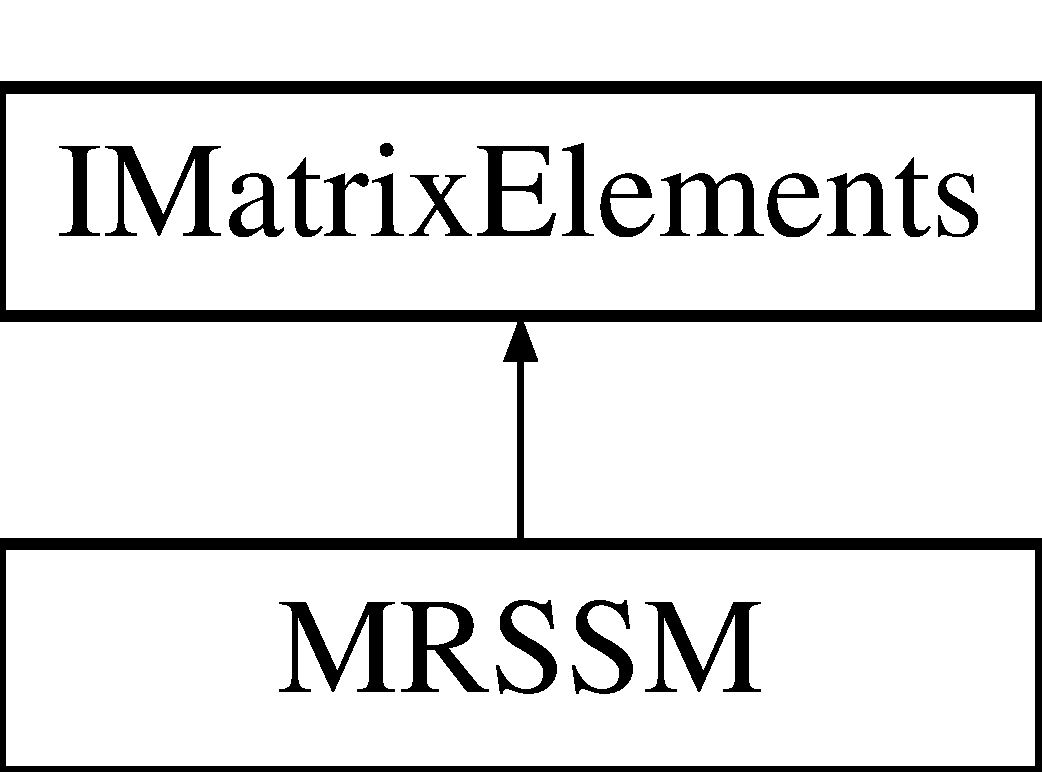
\includegraphics[height=2.000000cm]{classMRSSM}
\end{center}
\end{figure}
\subsection*{Public Member Functions}
\begin{DoxyCompactItemize}
\item 
\mbox{\Hypertarget{classMRSSM_a3f485c123c2d3efed9ec9950db329815}\label{classMRSSM_a3f485c123c2d3efed9ec9950db329815}} 
{\bfseries M\+R\+S\+SM} (boost\+::property\+\_\+tree\+::ptree const \&pt)
\item 
\mbox{\Hypertarget{classMRSSM_a4bf29333db6df3962e1f96873af1e8a1}\label{classMRSSM_a4bf29333db6df3962e1f96873af1e8a1}} 
double {\bfseries Born\+ME} (std\+::vector$<$ Particle $>$, double, double) const noexcept
\item 
\mbox{\Hypertarget{classMRSSM_a4b21e302b6f3cf4d8c417a0282468709}\label{classMRSSM_a4b21e302b6f3cf4d8c417a0282468709}} 
double {\bfseries Born\+C\+C\+ME} (std\+::vector$<$ Particle $>$, int, int, Eps\+Ord, std\+::vector$<$ \hyperlink{classVec4D}{Vec4D}$<$ double $>$$>$ const \&) const noexcept
\item 
\mbox{\Hypertarget{classMRSSM_aab207a9ec80cd70299012cd19cfbf96f}\label{classMRSSM_aab207a9ec80cd70299012cd19cfbf96f}} 
double {\bfseries Virtual\+ME} (std\+::vector$<$ Particle $>$, Eps\+Ord, double, double) const noexcept
\item 
\mbox{\Hypertarget{classMRSSM_ab89a86a500c8946a477ec8f6bdd2fba5}\label{classMRSSM_ab89a86a500c8946a477ec8f6bdd2fba5}} 
double {\bfseries Real\+ME} (std\+::vector$<$ Particle $>$, std\+::vector$<$ \hyperlink{classVec4D}{Vec4D}$<$ double $>$$>$ const \&) const noexcept
\end{DoxyCompactItemize}
\subsection*{Protected Attributes}
\begin{DoxyCompactItemize}
\item 
\mbox{\Hypertarget{classMRSSM_a7b4710a7a57255e9901935edbbf78ec4}\label{classMRSSM_a7b4710a7a57255e9901935edbbf78ec4}} 
const double {\bfseries MasssigmaO}
\item 
\mbox{\Hypertarget{classMRSSM_ac29fb0344519ace1517006a8a0e976b9}\label{classMRSSM_ac29fb0344519ace1517006a8a0e976b9}} 
const double {\bfseries MassphiO}
\item 
\mbox{\Hypertarget{classMRSSM_a64d0f4a9a892e39c6c5e621415b798d6}\label{classMRSSM_a64d0f4a9a892e39c6c5e621415b798d6}} 
const double {\bfseries Mass\+Glu}
\item 
\mbox{\Hypertarget{classMRSSM_a3246523a0f6aee64e351050e69b5809c}\label{classMRSSM_a3246523a0f6aee64e351050e69b5809c}} 
const double {\bfseries Mass\+Top}
\item 
\mbox{\Hypertarget{classMRSSM_aa1760b2961db89e6de0ca6dc009f8408}\label{classMRSSM_aa1760b2961db89e6de0ca6dc009f8408}} 
const double {\bfseries Mass\+SuL}
\item 
\mbox{\Hypertarget{classMRSSM_a509514932bc269192aad80eb334f23de}\label{classMRSSM_a509514932bc269192aad80eb334f23de}} 
const double {\bfseries Mass\+SuR}
\item 
\mbox{\Hypertarget{classMRSSM_a14346aebba69de118194328c4b9e63f8}\label{classMRSSM_a14346aebba69de118194328c4b9e63f8}} 
const double {\bfseries Mass\+SdL}
\item 
\mbox{\Hypertarget{classMRSSM_aa0abffb21c05ad2576f6363089cc87af}\label{classMRSSM_aa0abffb21c05ad2576f6363089cc87af}} 
const double {\bfseries Mass\+SdR}
\item 
\mbox{\Hypertarget{classMRSSM_a876d5e9376a4d9d148e2acba28ee7064}\label{classMRSSM_a876d5e9376a4d9d148e2acba28ee7064}} 
const double {\bfseries Mass\+SsL}
\item 
\mbox{\Hypertarget{classMRSSM_ae74e9ef756b9652e732327ffad1e7f46}\label{classMRSSM_ae74e9ef756b9652e732327ffad1e7f46}} 
const double {\bfseries Mass\+SsR}
\item 
\mbox{\Hypertarget{classMRSSM_aca2ef837460d4de9e176759ca0300eb2}\label{classMRSSM_aca2ef837460d4de9e176759ca0300eb2}} 
const double {\bfseries Mass\+ScL}
\item 
\mbox{\Hypertarget{classMRSSM_acc25487cacdae102618670a9efe7d1fc}\label{classMRSSM_acc25487cacdae102618670a9efe7d1fc}} 
const double {\bfseries Mass\+ScR}
\item 
\mbox{\Hypertarget{classMRSSM_ad86ae120c917f88aa7c8934d1fef2578}\label{classMRSSM_ad86ae120c917f88aa7c8934d1fef2578}} 
const double {\bfseries Mass\+SbL}
\item 
\mbox{\Hypertarget{classMRSSM_afd5778cd739891671f08595ec86e31aa}\label{classMRSSM_afd5778cd739891671f08595ec86e31aa}} 
const double {\bfseries Mass\+SbR}
\item 
\mbox{\Hypertarget{classMRSSM_ab3ae713607144c4b30a37fde2c32e468}\label{classMRSSM_ab3ae713607144c4b30a37fde2c32e468}} 
const double {\bfseries Mass\+StL}
\item 
\mbox{\Hypertarget{classMRSSM_ac4c1a53eece41e0cfd7ae40b21ee8523}\label{classMRSSM_ac4c1a53eece41e0cfd7ae40b21ee8523}} 
const double {\bfseries Mass\+StR}
\end{DoxyCompactItemize}
\subsection*{Additional Inherited Members}


The documentation for this class was generated from the following file\+:\begin{DoxyCompactItemize}
\item 
/home/wojciechk1/\+Programowanie/c++/rsymsqcd/include/M\+R\+S\+S\+M.\+h\end{DoxyCompactItemize}

\hypertarget{classMSSM}{}\section{M\+S\+SM Class Reference}
\label{classMSSM}\index{M\+S\+SM@{M\+S\+SM}}
Inheritance diagram for M\+S\+SM\+:\begin{figure}[H]
\begin{center}
\leavevmode
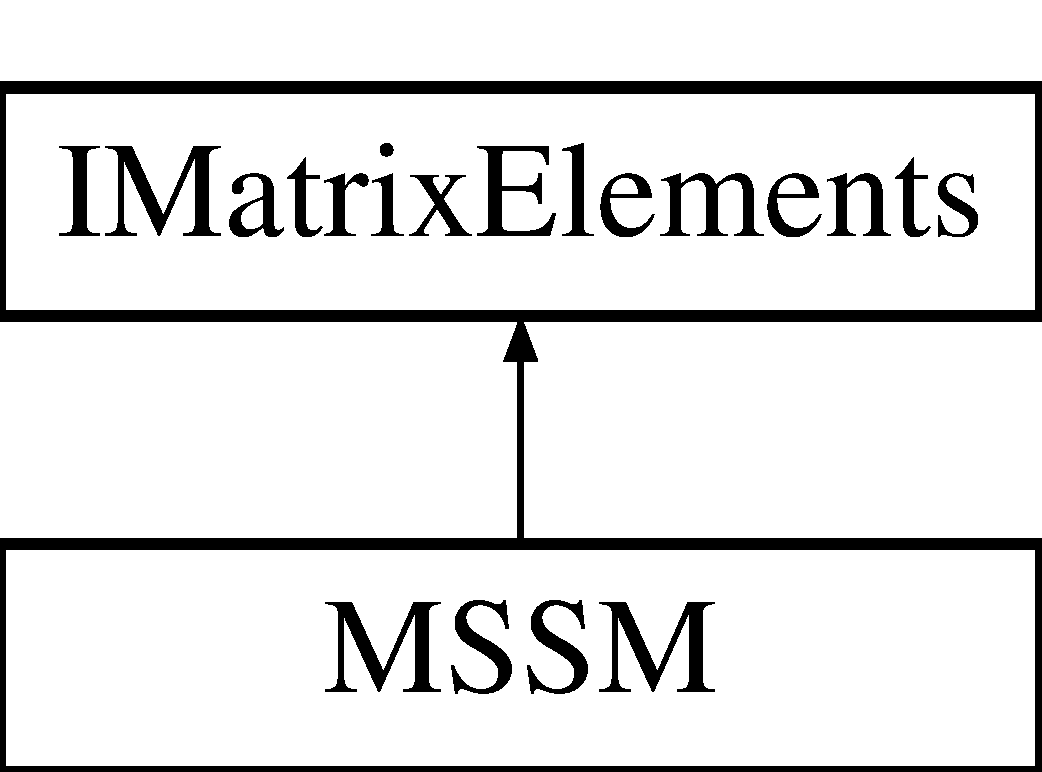
\includegraphics[height=2.000000cm]{classMSSM}
\end{center}
\end{figure}
\subsection*{Public Member Functions}
\begin{DoxyCompactItemize}
\item 
\mbox{\Hypertarget{classMSSM_a37c98e03fcb404dc5b5b9ed7b6672659}\label{classMSSM_a37c98e03fcb404dc5b5b9ed7b6672659}} 
{\bfseries M\+S\+SM} (boost\+::property\+\_\+tree\+::ptree const \&)
\item 
\mbox{\Hypertarget{classMSSM_a36406c9e5fadfa972f1cea93e1ad27c2}\label{classMSSM_a36406c9e5fadfa972f1cea93e1ad27c2}} 
double {\bfseries Born\+ME} (std\+::vector$<$ Particle $>$, double, double) const noexcept
\item 
\mbox{\Hypertarget{classMSSM_ac3ae0219b18c5e588ef94fbc6ace4c5e}\label{classMSSM_ac3ae0219b18c5e588ef94fbc6ace4c5e}} 
double {\bfseries Born\+C\+C\+ME} (std\+::vector$<$ Particle $>$, int, int, Eps\+Ord, std\+::vector$<$ \hyperlink{classVec4D}{Vec4D}$<$ double $>$$>$ const \&) const noexcept
\item 
\mbox{\Hypertarget{classMSSM_a05c93f6672f90df48f2af8a2f5261950}\label{classMSSM_a05c93f6672f90df48f2af8a2f5261950}} 
double {\bfseries Virtual\+ME} (std\+::vector$<$ Particle $>$, Eps\+Ord, double, double) const noexcept
\item 
\mbox{\Hypertarget{classMSSM_a94cbeecf337257efe49db8a4407559d0}\label{classMSSM_a94cbeecf337257efe49db8a4407559d0}} 
double {\bfseries Real\+ME} (std\+::vector$<$ Particle $>$, std\+::vector$<$ \hyperlink{classVec4D}{Vec4D}$<$ double $>$$>$ const \&) const noexcept
\end{DoxyCompactItemize}
\subsection*{Additional Inherited Members}


The documentation for this class was generated from the following file\+:\begin{DoxyCompactItemize}
\item 
/home/wojciechk1/\+Programowanie/c++/rsymsqcd/include/M\+S\+S\+M.\+h\end{DoxyCompactItemize}

\hypertarget{classProcess}{}\section{Process Class Reference}
\label{classProcess}\index{Process@{Process}}
\subsection*{Public Member Functions}
\begin{DoxyCompactItemize}
\item 
\mbox{\Hypertarget{classProcess_a1c62627941d43a632a2ba72edde8441b}\label{classProcess_a1c62627941d43a632a2ba72edde8441b}} 
{\bfseries Process} (std\+::string, boost\+::property\+\_\+tree\+::ptree)
\end{DoxyCompactItemize}
\subsection*{Public Attributes}
\begin{DoxyCompactItemize}
\item 
\mbox{\Hypertarget{classProcess_acf97a283d10f81f42c09fb10c271b9fe}\label{classProcess_acf97a283d10f81f42c09fb10c271b9fe}} 
double(Process\+::$\ast$ {\bfseries matrixelement\+Tree} )(double, double) const
\item 
\mbox{\Hypertarget{classProcess_a6959adc59277bbc489d61acc6ace9f3e}\label{classProcess_a6959adc59277bbc489d61acc6ace9f3e}} 
double(Process\+::$\ast$ {\bfseries sigma\+Part\+Tree1} )(double)
\item 
\mbox{\Hypertarget{classProcess_a27b2b360a232bc072abe0acf511123c3}\label{classProcess_a27b2b360a232bc072abe0acf511123c3}} 
double(Process\+::$\ast$ {\bfseries sigma\+Part\+Tree2} )(double)
\item 
\mbox{\Hypertarget{classProcess_a96055c754e57a308742e94cc2eb5341c}\label{classProcess_a96055c754e57a308742e94cc2eb5341c}} 
std\+::array$<$ double, 2 $>$(Process\+::$\ast$ {\bfseries splitting\+\_\+kernel1} )(double) const noexcept
\item 
\mbox{\Hypertarget{classProcess_ac5392ca07448c1b08c8513456165d5ee}\label{classProcess_ac5392ca07448c1b08c8513456165d5ee}} 
std\+::array$<$ double, 2 $>$(Process\+::$\ast$ {\bfseries splitting\+\_\+kernel2} )(double) const noexcept
\item 
\mbox{\Hypertarget{classProcess_aebcafc03257ff5aeca1a3a25e0bd88fe}\label{classProcess_aebcafc03257ff5aeca1a3a25e0bd88fe}} 
double(Process\+::$\ast$ {\bfseries matrixelement\+Virt} )(double, double, double, double, int)
\item 
\mbox{\Hypertarget{classProcess_ae3fcf76ca5dda1c3c44f6308eca25b44}\label{classProcess_ae3fcf76ca5dda1c3c44f6308eca25b44}} 
double(Process\+::$\ast$ {\bfseries matrixelement\+Real\+\_\+\+SC} )(double, double)
\item 
\mbox{\Hypertarget{classProcess_a89b2b63998f4401e9e97eebf9694ac25}\label{classProcess_a89b2b63998f4401e9e97eebf9694ac25}} 
double(Process\+::$\ast$ {\bfseries matrixelement\+Real\+\_\+\+H\+C1} )(double, double, double)
\item 
\mbox{\Hypertarget{classProcess_a2d8b6a1029ed9ea4d5cf96fdd14a53e3}\label{classProcess_a2d8b6a1029ed9ea4d5cf96fdd14a53e3}} 
double(Process\+::$\ast$ {\bfseries matrixelement\+Real\+\_\+\+H\+C2} )(double, double, double)
\item 
\mbox{\Hypertarget{classProcess_aa9861c9231581fd9a17f6ff14885e64a}\label{classProcess_aa9861c9231581fd9a17f6ff14885e64a}} 
double(Process\+::$\ast$ {\bfseries matrixelement\+Real\+\_\+\+HnonC} )(const std\+::vector$<$ double $\ast$ $>$ \&) const
\item 
\mbox{\Hypertarget{classProcess_ad6133fbfba8ef70546c53c9010dafdc1}\label{classProcess_ad6133fbfba8ef70546c53c9010dafdc1}} 
double(Process\+::$\ast$ {\bfseries matrixelement\+Real\+\_\+\+Hnon\+C\+\_\+\+C\+Sub1} )(const std\+::vector$<$ double $\ast$ $>$ \&) const noexcept
\item 
\mbox{\Hypertarget{classProcess_aa735bcf530026221f049f102322c8663}\label{classProcess_aa735bcf530026221f049f102322c8663}} 
double(Process\+::$\ast$ {\bfseries matrixelement\+Real\+\_\+\+Hnon\+C\+\_\+\+C\+Sub2} )(const std\+::vector$<$ double $\ast$ $>$ \&) const noexcept
\item 
\mbox{\Hypertarget{classProcess_ae6061019e1064a2432eee55d2328fba6}\label{classProcess_ae6061019e1064a2432eee55d2328fba6}} 
double {\bfseries m1}
\item 
\mbox{\Hypertarget{classProcess_a41cd2505bff11029ebfb9d0c0eba6ede}\label{classProcess_a41cd2505bff11029ebfb9d0c0eba6ede}} 
double {\bfseries m2}
\item 
\mbox{\Hypertarget{classProcess_a3f78ea46255307582d1e307ae313849b}\label{classProcess_a3f78ea46255307582d1e307ae313849b}} 
double {\bfseries c1}
\item 
\mbox{\Hypertarget{classProcess_a96dc47c8f523deadce142b932368b48b}\label{classProcess_a96dc47c8f523deadce142b932368b48b}} 
double {\bfseries c2}
\item 
\mbox{\Hypertarget{classProcess_a49ef9dba94bed258c341478a23b0ec34}\label{classProcess_a49ef9dba94bed258c341478a23b0ec34}} 
double {\bfseries c3}
\item 
\mbox{\Hypertarget{classProcess_ae2b68f8da651b064da1ed312d689fcb8}\label{classProcess_ae2b68f8da651b064da1ed312d689fcb8}} 
double {\bfseries c4}
\item 
\mbox{\Hypertarget{classProcess_ac00a109bebb0ef93f0b254a0ab708de6}\label{classProcess_ac00a109bebb0ef93f0b254a0ab708de6}} 
double {\bfseries k}
\item 
\mbox{\Hypertarget{classProcess_ae15ca69e10cabf342b2b653ddf4d2076}\label{classProcess_ae15ca69e10cabf342b2b653ddf4d2076}} 
double {\bfseries h}
\item 
\mbox{\Hypertarget{classProcess_ac1eb1e163b010b3044fb464213f053b8}\label{classProcess_ac1eb1e163b010b3044fb464213f053b8}} 
bool {\bfseries partonic}
\item 
\mbox{\Hypertarget{classProcess_aeb33669fd7dc8c84321f2e26c796a0f9}\label{classProcess_aeb33669fd7dc8c84321f2e26c796a0f9}} 
std\+::vector$<$ std\+::vector$<$ int $>$ $>$ {\bfseries flav}
\end{DoxyCompactItemize}


The documentation for this class was generated from the following file\+:\begin{DoxyCompactItemize}
\item 
/home/wojciechk1/\+Programowanie/c++/rsymsqcd/include/Process.\+hpp\end{DoxyCompactItemize}

\hypertarget{classSM}{}\section{SM Class Reference}
\label{classSM}\index{SM@{SM}}
Inheritance diagram for SM\+:\begin{figure}[H]
\begin{center}
\leavevmode
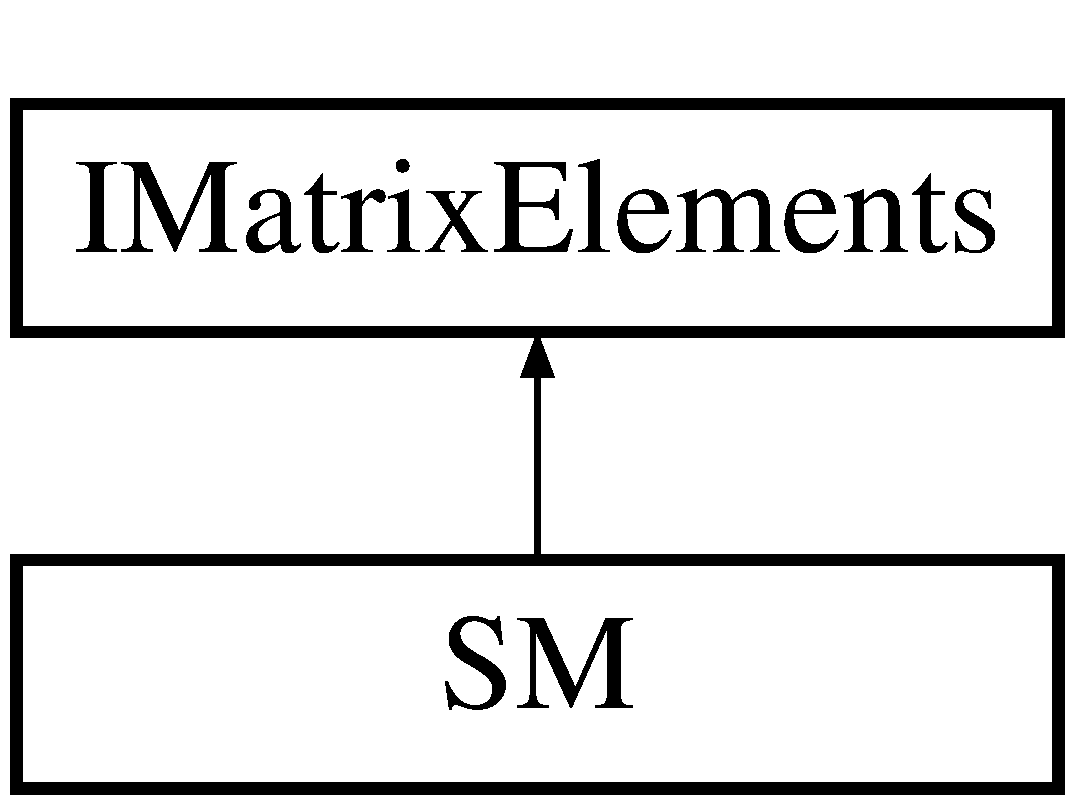
\includegraphics[height=2.000000cm]{classSM}
\end{center}
\end{figure}
\subsection*{Public Member Functions}
\begin{DoxyCompactItemize}
\item 
\mbox{\Hypertarget{classSM_ae0cdbc17b42976fdc2b98aa80f5f21f0}\label{classSM_ae0cdbc17b42976fdc2b98aa80f5f21f0}} 
{\bfseries SM} (boost\+::property\+\_\+tree\+::ptree const \&ptree)
\item 
\mbox{\Hypertarget{classSM_a204b9b1ba61483555f49778a71b00701}\label{classSM_a204b9b1ba61483555f49778a71b00701}} 
double {\bfseries Born\+ME} (std\+::vector$<$ Particle $>$, double, double) const noexcept
\item 
\mbox{\Hypertarget{classSM_a1bad8844522622c280374c7086f25b03}\label{classSM_a1bad8844522622c280374c7086f25b03}} 
double {\bfseries Born\+C\+C\+ME} (std\+::vector$<$ Particle $>$, int, int, Eps\+Ord, std\+::vector$<$ \hyperlink{classVec4D}{Vec4D}$<$ double $>$$>$ const \&) const noexcept
\item 
\mbox{\Hypertarget{classSM_aeb5e31743d6bfbdafb7370a46f110f95}\label{classSM_aeb5e31743d6bfbdafb7370a46f110f95}} 
double {\bfseries Virtual\+ME} (std\+::vector$<$ Particle $>$, Eps\+Ord, double, double) const noexcept
\item 
\mbox{\Hypertarget{classSM_abd546052316e2c8a323b40495bcdb461}\label{classSM_abd546052316e2c8a323b40495bcdb461}} 
double {\bfseries Real\+ME} (std\+::vector$<$ Particle $>$, std\+::vector$<$ \hyperlink{classVec4D}{Vec4D}$<$ double $>$$>$ const \&) const noexcept
\end{DoxyCompactItemize}
\subsection*{Additional Inherited Members}


The documentation for this class was generated from the following file\+:\begin{DoxyCompactItemize}
\item 
/home/wojciechk1/\+Programowanie/c++/rsymsqcd/include/S\+M.\+h\end{DoxyCompactItemize}

\hypertarget{classVec4D}{}\section{Vec4D$<$ T $>$ Class Template Reference}
\label{classVec4D}\index{Vec4\+D$<$ T $>$@{Vec4\+D$<$ T $>$}}
\subsection*{Public Member Functions}
\begin{DoxyCompactItemize}
\item 
\mbox{\Hypertarget{classVec4D_af7fd3d505e4ee71963da32d4738a3721}\label{classVec4D_af7fd3d505e4ee71963da32d4738a3721}} 
{\bfseries Vec4D} (const \hyperlink{classVec4D}{Vec4D}$<$ T $>$ \&)=default
\item 
\mbox{\Hypertarget{classVec4D_aa9aa821a1d139e83672efdb1a497d829}\label{classVec4D_aa9aa821a1d139e83672efdb1a497d829}} 
\hyperlink{classVec4D}{Vec4D}$<$ T $>$ {\bfseries operator=} (const \hyperlink{classVec4D}{Vec4D}$<$ T $>$ \&)
\item 
\mbox{\Hypertarget{classVec4D_a417cd8a1639f6a9e8b478d837a057db6}\label{classVec4D_a417cd8a1639f6a9e8b478d837a057db6}} 
{\bfseries Vec4D} (T t, T x, T y, T z)
\end{DoxyCompactItemize}
\subsection*{Public Attributes}
\begin{DoxyCompactItemize}
\item 
\mbox{\Hypertarget{classVec4D_a2a0096c956b91a72261ca940d9210efc}\label{classVec4D_a2a0096c956b91a72261ca940d9210efc}} 
T {\bfseries t\+\_\+}
\item 
\mbox{\Hypertarget{classVec4D_aa9a006cc20d8ff45c9bb98c282a93776}\label{classVec4D_aa9a006cc20d8ff45c9bb98c282a93776}} 
T {\bfseries x\+\_\+}
\item 
\mbox{\Hypertarget{classVec4D_a98a9fe30736359383dd5c10b2a31a4bc}\label{classVec4D_a98a9fe30736359383dd5c10b2a31a4bc}} 
T {\bfseries y\+\_\+}
\item 
\mbox{\Hypertarget{classVec4D_a0b22629bd0e4ec4774df3310eea443f4}\label{classVec4D_a0b22629bd0e4ec4774df3310eea443f4}} 
T {\bfseries z\+\_\+}
\end{DoxyCompactItemize}


The documentation for this class was generated from the following file\+:\begin{DoxyCompactItemize}
\item 
/home/wojciechk1/\+Programowanie/c++/rsymsqcd/include/Vec4\+D.\+hpp\end{DoxyCompactItemize}

\hypertarget{classXSection}{}\section{X\+Section Class Reference}
\label{classXSection}\index{X\+Section@{X\+Section}}
Inheritance diagram for X\+Section\+:\begin{figure}[H]
\begin{center}
\leavevmode
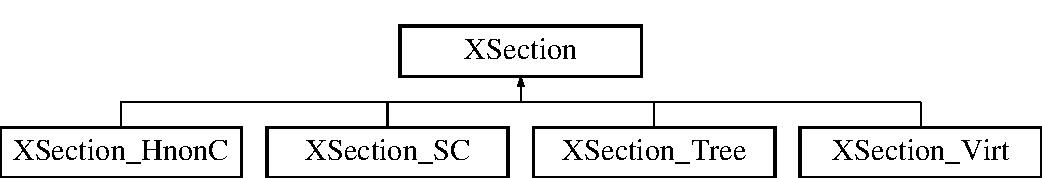
\includegraphics[height=2.000000cm]{classXSection}
\end{center}
\end{figure}
\subsection*{Public Member Functions}
\begin{DoxyCompactItemize}
\item 
\mbox{\Hypertarget{classXSection_ad697c9f68154808c927267666e8a1d37}\label{classXSection_ad697c9f68154808c927267666e8a1d37}} 
virtual std\+::array$<$ double, 3 $>$ {\bfseries integrate} ()=0
\end{DoxyCompactItemize}
\subsection*{Static Public Member Functions}
\begin{DoxyCompactItemize}
\item 
\mbox{\Hypertarget{classXSection_a6cc33979c6bb62f6812a7e3768f84032}\label{classXSection_a6cc33979c6bb62f6812a7e3768f84032}} 
static void {\bfseries init} (boost\+::property\+\_\+tree\+::ptree, boost\+::program\+\_\+options\+::variables\+\_\+map)
\end{DoxyCompactItemize}
\subsection*{Static Protected Attributes}
\begin{DoxyCompactItemize}
\item 
\mbox{\Hypertarget{classXSection_a239a2db2356100d83eafb9026ec5d129}\label{classXSection_a239a2db2356100d83eafb9026ec5d129}} 
static std\+::vector$<$ std\+::vector$<$ Particle $>$ $>$ {\bfseries particles}
\item 
\mbox{\Hypertarget{classXSection_ada3e26fe411954e55d36ba3768a7ff79}\label{classXSection_ada3e26fe411954e55d36ba3768a7ff79}} 
static \hyperlink{classIMatrixElements}{I\+Matrix\+Elements} $\ast$ {\bfseries model}
\item 
\mbox{\Hypertarget{classXSection_adda4e44d677508d6f437db1e43db2861}\label{classXSection_adda4e44d677508d6f437db1e43db2861}} 
static double {\bfseries dS}
\item 
\mbox{\Hypertarget{classXSection_ad31c69a4dcde5f7050d627db5ed0475c}\label{classXSection_ad31c69a4dcde5f7050d627db5ed0475c}} 
static double {\bfseries dC}
\item 
\mbox{\Hypertarget{classXSection_a50569ac12be53de5400bd51a885b66b8}\label{classXSection_a50569ac12be53de5400bd51a885b66b8}} 
static boost\+::property\+\_\+tree\+::ptree {\bfseries pt}
\item 
\mbox{\Hypertarget{classXSection_a9b7d8b14ca35b4d41ee786b125f1cad4}\label{classXSection_a9b7d8b14ca35b4d41ee786b125f1cad4}} 
static boost\+::program\+\_\+options\+::variables\+\_\+map {\bfseries vm}
\item 
\mbox{\Hypertarget{classXSection_a52631134ca09ca4acd54ba712eae6a4a}\label{classXSection_a52631134ca09ca4acd54ba712eae6a4a}} 
static double {\bfseries S\+\_\+sqrt}
\item 
\mbox{\Hypertarget{classXSection_a7f414ef300c0cdc284bd833b473d537a}\label{classXSection_a7f414ef300c0cdc284bd833b473d537a}} 
static double {\bfseries S}
\item 
\mbox{\Hypertarget{classXSection_aeb6572d9b7a49f9d76e16d81977a95ee}\label{classXSection_aeb6572d9b7a49f9d76e16d81977a95ee}} 
static double {\bfseries mu\+\_\+r}
\item 
\mbox{\Hypertarget{classXSection_ad85662a63c6a9082be158468618c1cfc}\label{classXSection_ad85662a63c6a9082be158468618c1cfc}} 
static double {\bfseries mu\+\_\+f}
\item 
\mbox{\Hypertarget{classXSection_a2a6abdf1668eb3582ca0b92b9720aa0f}\label{classXSection_a2a6abdf1668eb3582ca0b92b9720aa0f}} 
static double {\bfseries m1}
\item 
\mbox{\Hypertarget{classXSection_af1ce6a64797281650b1e3884ab14b685}\label{classXSection_af1ce6a64797281650b1e3884ab14b685}} 
static double {\bfseries m2}
\item 
\mbox{\Hypertarget{classXSection_a6ca6de511db7290694dbf23bcd379e6b}\label{classXSection_a6ca6de511db7290694dbf23bcd379e6b}} 
static const L\+H\+A\+P\+D\+F\+::\+P\+DF $\ast$ {\bfseries pdf}
\end{DoxyCompactItemize}


The documentation for this class was generated from the following files\+:\begin{DoxyCompactItemize}
\item 
/home/wojciechk1/\+Programowanie/c++/rsymsqcd/include/X\+Section.\+hpp\item 
/home/wojciechk1/\+Programowanie/c++/rsymsqcd/src/main.\+cpp\item 
/home/wojciechk1/\+Programowanie/c++/rsymsqcd/src/X\+Section.\+cpp\end{DoxyCompactItemize}

\hypertarget{classXSection__HnonC}{}\section{X\+Section\+\_\+\+HnonC Class Reference}
\label{classXSection__HnonC}\index{X\+Section\+\_\+\+HnonC@{X\+Section\+\_\+\+HnonC}}
Inheritance diagram for X\+Section\+\_\+\+HnonC\+:\begin{figure}[H]
\begin{center}
\leavevmode
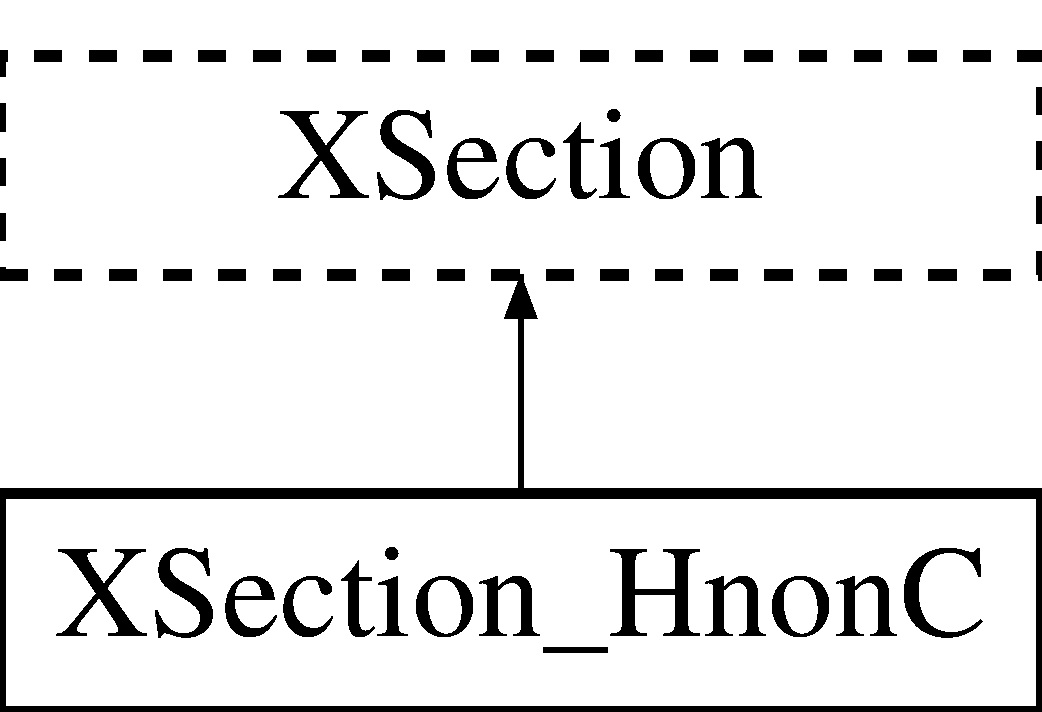
\includegraphics[height=2.000000cm]{classXSection__HnonC}
\end{center}
\end{figure}
\subsection*{Public Member Functions}
\begin{DoxyCompactItemize}
\item 
\mbox{\Hypertarget{classXSection__HnonC_a5eef4450e024b498769ff1d02ec4cdd6}\label{classXSection__HnonC_a5eef4450e024b498769ff1d02ec4cdd6}} 
std\+::array$<$ double, 3 $>$ {\bfseries integrate} ()
\end{DoxyCompactItemize}
\subsection*{Static Public Attributes}
\begin{DoxyCompactItemize}
\item 
\mbox{\Hypertarget{classXSection__HnonC_aa578c0b49a19199ded7783b3e9457ad7}\label{classXSection__HnonC_aa578c0b49a19199ded7783b3e9457ad7}} 
static std\+::vector$<$ \hyperlink{classCSDipole}{C\+S\+Dipole} $>$ {\bfseries cs\+\_\+dipoles}
\end{DoxyCompactItemize}
\subsection*{Additional Inherited Members}


The documentation for this class was generated from the following files\+:\begin{DoxyCompactItemize}
\item 
/home/wojciechk1/\+Programowanie/c++/rsymsqcd/include/X\+Section\+\_\+\+Hnon\+C.\+hpp\item 
/home/wojciechk1/\+Programowanie/c++/rsymsqcd/src/X\+Section\+\_\+\+Hnon\+C.\+cpp\end{DoxyCompactItemize}

\hypertarget{classXSection__SC}{}\section{X\+Section\+\_\+\+SC Class Reference}
\label{classXSection__SC}\index{X\+Section\+\_\+\+SC@{X\+Section\+\_\+\+SC}}
Inheritance diagram for X\+Section\+\_\+\+SC\+:\begin{figure}[H]
\begin{center}
\leavevmode
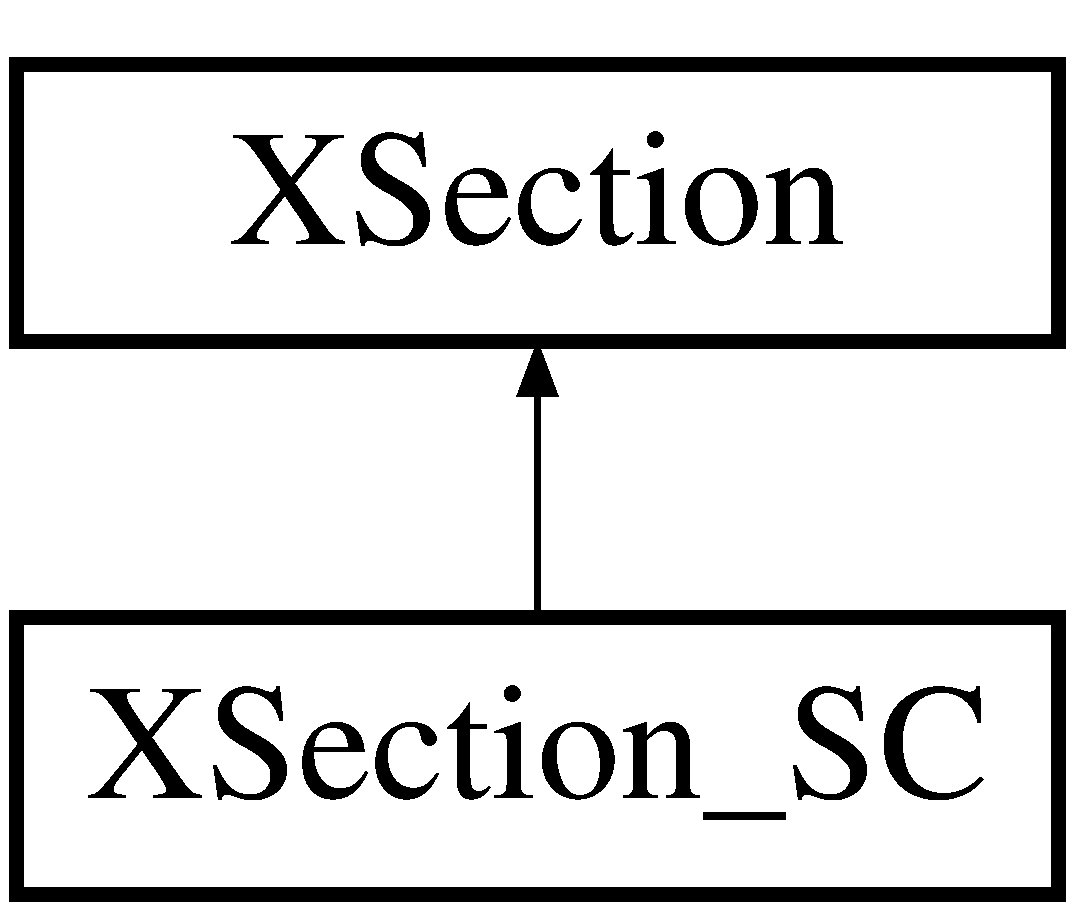
\includegraphics[height=2.000000cm]{classXSection__SC}
\end{center}
\end{figure}
\subsection*{Public Member Functions}
\begin{DoxyCompactItemize}
\item 
\mbox{\Hypertarget{classXSection__SC_af1dd47bccac55582b219cd99458e311e}\label{classXSection__SC_af1dd47bccac55582b219cd99458e311e}} 
std\+::array$<$ double, 3 $>$ {\bfseries integrate} ()
\end{DoxyCompactItemize}
\subsection*{Static Public Member Functions}
\begin{DoxyCompactItemize}
\item 
\mbox{\Hypertarget{classXSection__SC_a49b7b2b591948a17b4133397c41ae290}\label{classXSection__SC_a49b7b2b591948a17b4133397c41ae290}} 
static double {\bfseries f} (double $\ast$, double $\ast$, double $\ast$, double $\ast$)
\end{DoxyCompactItemize}
\subsection*{Static Public Attributes}
\begin{DoxyCompactItemize}
\item 
\mbox{\Hypertarget{classXSection__SC_ac00d0eca18be8844a136d3bd335eb7da}\label{classXSection__SC_ac00d0eca18be8844a136d3bd335eb7da}} 
static std\+::vector$<$ \hyperlink{classCSDipole}{C\+S\+Dipole} $>$ {\bfseries cs\+\_\+dipoles}
\end{DoxyCompactItemize}
\subsection*{Additional Inherited Members}


The documentation for this class was generated from the following files\+:\begin{DoxyCompactItemize}
\item 
/home/wojciechk1/\+Programowanie/c++/rsymsqcd/include/X\+Section\+\_\+\+S\+C.\+hpp\item 
/home/wojciechk1/\+Programowanie/c++/rsymsqcd/src/X\+Section\+\_\+\+S\+C.\+cpp\end{DoxyCompactItemize}

\hypertarget{classXSection__Tree}{}\section{X\+Section\+\_\+\+Tree Class Reference}
\label{classXSection__Tree}\index{X\+Section\+\_\+\+Tree@{X\+Section\+\_\+\+Tree}}
Inheritance diagram for X\+Section\+\_\+\+Tree\+:\begin{figure}[H]
\begin{center}
\leavevmode
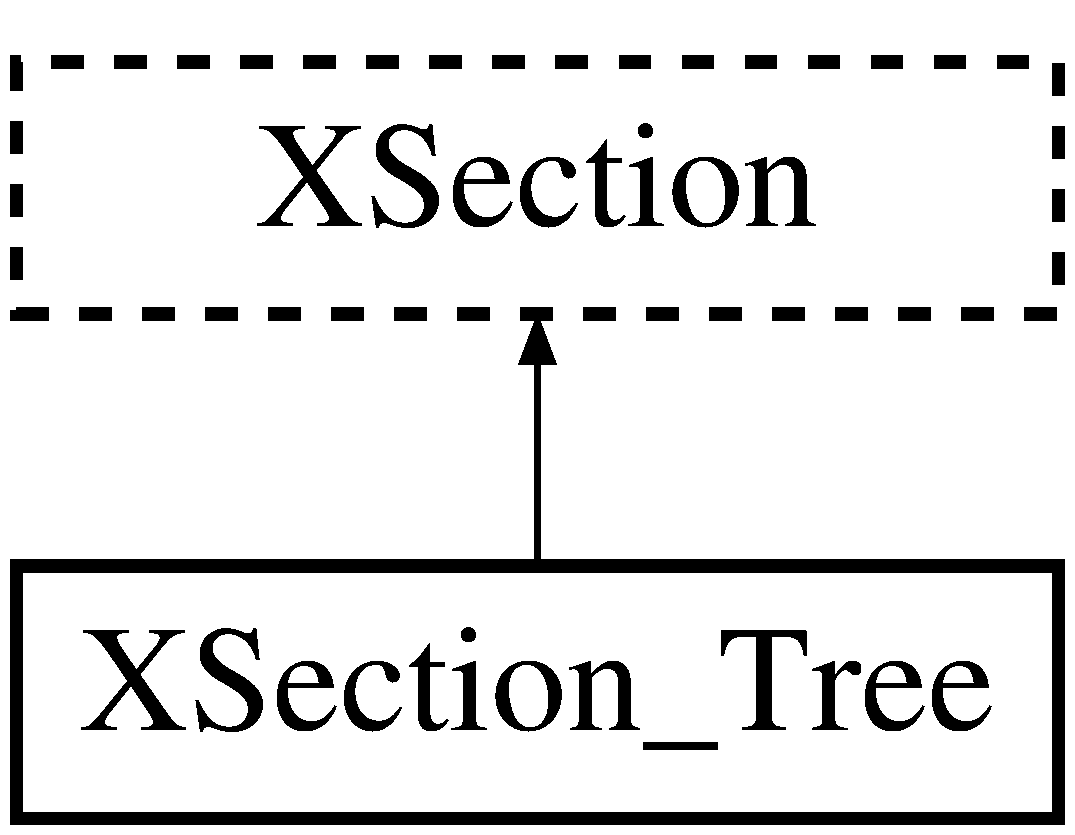
\includegraphics[height=2.000000cm]{classXSection__Tree}
\end{center}
\end{figure}
\subsection*{Public Member Functions}
\begin{DoxyCompactItemize}
\item 
\mbox{\Hypertarget{classXSection__Tree_a23fa57cf909c85640de9598e63285b14}\label{classXSection__Tree_a23fa57cf909c85640de9598e63285b14}} 
std\+::array$<$ double, 3 $>$ {\bfseries integrate} ()
\item 
\mbox{\Hypertarget{classXSection__Tree_adcdb3a71719870771d3c863dc41dc20a}\label{classXSection__Tree_adcdb3a71719870771d3c863dc41dc20a}} 
void {\bfseries show\+\_\+settings} ()
\end{DoxyCompactItemize}
\subsection*{Additional Inherited Members}


The documentation for this class was generated from the following files\+:\begin{DoxyCompactItemize}
\item 
/home/wojciechk1/\+Programowanie/c++/rsymsqcd/include/X\+Section\+\_\+\+Tree.\+hpp\item 
/home/wojciechk1/\+Programowanie/c++/rsymsqcd/src/X\+Section\+\_\+\+Tree.\+cpp\end{DoxyCompactItemize}

\hypertarget{classXSection__Virt}{}\section{X\+Section\+\_\+\+Virt Class Reference}
\label{classXSection__Virt}\index{X\+Section\+\_\+\+Virt@{X\+Section\+\_\+\+Virt}}
Inheritance diagram for X\+Section\+\_\+\+Virt\+:\begin{figure}[H]
\begin{center}
\leavevmode
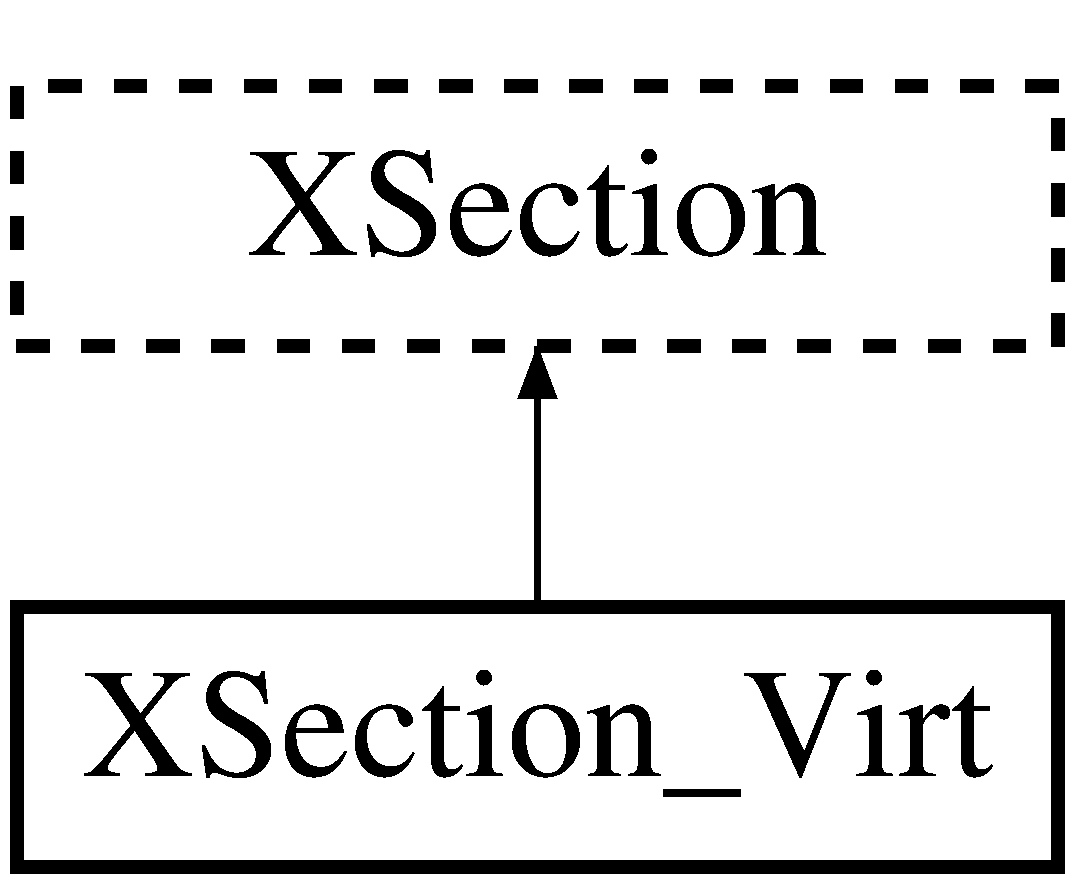
\includegraphics[height=2.000000cm]{classXSection__Virt}
\end{center}
\end{figure}
\subsection*{Public Member Functions}
\begin{DoxyCompactItemize}
\item 
\mbox{\Hypertarget{classXSection__Virt_a5a691c6860054b2608b234c9755a1fbb}\label{classXSection__Virt_a5a691c6860054b2608b234c9755a1fbb}} 
std\+::array$<$ double, 3 $>$ {\bfseries integrate} ()
\end{DoxyCompactItemize}
\subsection*{Static Public Attributes}
\begin{DoxyCompactItemize}
\item 
\mbox{\Hypertarget{classXSection__Virt_ae2d09c66ecbe84e262b2986a9665bc8b}\label{classXSection__Virt_ae2d09c66ecbe84e262b2986a9665bc8b}} 
static std\+::vector$<$ \hyperlink{classCSDipole}{C\+S\+Dipole} $>$ {\bfseries cs\+\_\+dipoles}
\end{DoxyCompactItemize}
\subsection*{Additional Inherited Members}


The documentation for this class was generated from the following files\+:\begin{DoxyCompactItemize}
\item 
/home/wojciechk1/\+Programowanie/c++/rsymsqcd/include/X\+Section\+\_\+\+Virt.\+hpp\item 
/home/wojciechk1/\+Programowanie/c++/rsymsqcd/src/X\+Section\+\_\+\+Virt.\+cpp\end{DoxyCompactItemize}

%--- End generated contents ---

% Index
\backmatter
\newpage
\phantomsection
\clearemptydoublepage
\addcontentsline{toc}{chapter}{Index}
\printindex

\end{document}
